\section{Aplicación de ejemplo}

Para comprender mejor esta problemática veamos un ejemplo. Supongamos una simple
aplicación, donde los clientes de un banco pueden transferir dinero de
una cuenta a otra. Al realizar una transferencia, hay que extraer el monto
indicado de una cuenta, y depositarlo en otra. 
Al ejecutar cualquiera de estas dos operaciones se pueden producir errores,
como por ejemplo, que no haya saldo saldo suficiente, o que el depósito supere
el máximo permitido.
La  figura \ref{example} muestra el diagrama de clases de la aplicación de
ejemplo

	\begin{figure}[h]
		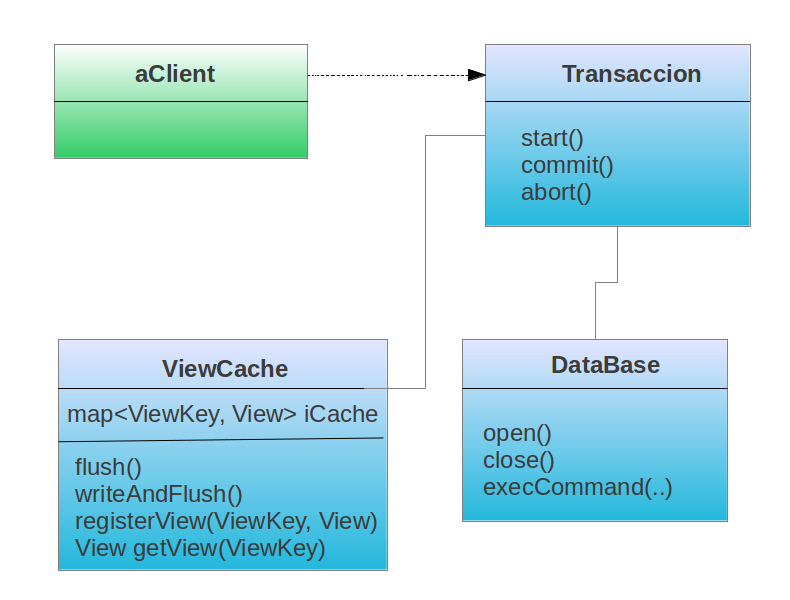
\includegraphics{img/objectTransaction}
		\caption{Diagrama UML de la aplicación de ejemplo}
		\label{example}
	\end{figure}	


El sistema me permite realizar múltiples transferencias a la vez y por último
realizar la confirmación o la cancelación de todas ellas. También brinda la posibilidad
de realizar múltiples transacciones, por ejemplo, en la edición de un cliente,
se puede editar, eliminar o crear cuentas. A su vez se puede hacer una
transferencia a otra cuenta. En cada una de esas operaciones se esta
trabajando en dentro de una transacción. y las operaciones pueden ser
canceladas por unidad, es decir, se cancelan o se confirman por transacción.

Caso de uso 1: transferir plata.
Tres ventajas:
- queda más simple
- menos posibilidad de mandármela
- concurrencia.

Poner el código como queda.

Caso de uso 2: transferencias múltiples.
muchas transferencias en una única transacción\ldots fijate si sale algo y si no
lo volamos.

\section{Nuestra herramienta: }

En esta sección se explica como se llevó a cabo la implementación de la solución
propuesta en la Sección \ref{sec:Solucion}, y cumpliendo el objetivo detallado
en la Sección \ref{sec:Objetivo}. Se desarrollaron dos herramientas
fundamentales para lo planteado. \emph{Pure Objects Observable} (POO) para atacar a la
problemática de la observabilidad y \emph{Pure Object Transaction} (POT) para
atacar a la problemática transaccional.
	
	\subsection{Selección de un framework de aspectos}  
	Un primer paso para la implementación de la herramienta fue la selección de una
	tecnología que permitiera desarrollar utilizando programación orientada a
	aspectos.
	Con ese objetivo, se evaluaron dos frameworks: Javassist \cite{??} y AspectJ
	\cite{KiczalesHHKPG01}.

	\medskip 
	Encontramos que AspectJ es una herramienta de más alto nivel, que extiende
	el lenguaje Java agregando construcciones específicas para trabajar con
	los conceptos de la teoría de programación orientada a aspectos.
	Por otro lado AspectJ requiere que el programador que use nuestro framework
	utilice un compilador específico. Consideramos que esta característica es muy
	negativa, por condicionar el entorno de trabajo de los usuarios de nuestra
	herramienta.
	En cambio Javassist agrega los aspectos al momento de la carga de las clases,
	sólo requiere que utilicemos un \emph{ClassLoader} específico.

	Elegimos Javassist por su menor impacto para el programador que utilice el
	framework como usuario.
	Para minimizar los problemas asociados a utilizar un framework de tan bajo
	nivel desarrollamos una herramienta que simplifica su uso agregando algunas
	abstracciones útiles. Esta herramienta se describe en la sección siguiente.

	\subsection{Desarrollo de Aspect for Pure Objects}

	El framework Javassist permite modificar directamente el \emph{bytecode} de
	una clase en el momento de cargarla.
	Por ser de tan bajo nivel es uno de los frameworks de aspectos más poderosos,
	pero a su vez el código se hace poco entendible.
	Por eso se desarrolló una herramienta llamada \emph{Aspect for Pure Objects} (APO), 
	que permite configurar aspectos utilizando conceptos de más alto nivel y
	aplicárselo a un grupo de objetos.
	
	La Figura \ref{bleh} muestra esquemáticamente el diseño de la herramienta.
	Una instancia de \code{AdviceWeaver} se ocupa de aplicar los cambios sobre las
	clases.
	Para ello cuenta con un conjunto de \code{Advice} que consisten de un
	\code{Predicate} (que determina el conjunto de clases sobre el que aplica el
	advice) y un objeto que implemente la interfaz \code{ExprEditor} (que
	será el responsable de realizar las modificaciones sobre
	las clases alcanzadas por el advice).
	Finalmente una instancia de \code{APOCrlassLoader}, instalada como class loader
	del sistema permite que antes de utilizar cualquier clase esta pueda ser procesada por el \code{AdviceWeaver}
	
	Para implementar las modificaciones se provee una implementación de
	\code{ExprEditor} que contiene una colección de modificaciones expresadas en un
	lenguaje de alto nivel y las traduce al lenguaje de bajo nivel que requiere el
	framework Javassist.
	La Figura \ref{??} muestra un ejemplo de código de este lenguaje de alto nivel,
	tomado del framework POO, que se describe en la Sección \ref{poo}.
	A su vez, la Tabla \ref{??} describe las expresiones propias del lenguaje
	definido por APO, su significado y su traducción al lenguaje de expresiones de
	Javassist.

	\begin{lstlisting}
		java.lang.Object oldValue = $oldValue; 
		$originalStatement
		$this.firePropertyChange('$fieldName', oldValue, $newValue);
	\end{lstlisting}
	
	\begin{tabular}{|c|c|p{6cm}|}
	\hline
	Expresión APO & Expresión Javassist & Significado \\
	\hline
	\$oldValue & ??? & El valor del atributo antes de la asignación que está siendo
	modificada.
	\\
	\hline
	\end{tabular} 
	
	\subsection{Pure Object Transaction}
		\label{pot} 
		Pure Object Transaction (POT) es la herramienta que implementa el aspecto
		transaccional como se definió en la sección \ref{aspectoTransaccional}.
		Está basado en una implementación anterior de Nicolás Passerini y Javier
		Fernandes, que se actualizó para aprovechar el framework APO y facilitar su
		integración con las demás herramientas desarrolladas.
		
		\medskip
		 
		Este framework intercepta todas las lecturas y escrituras de los atributos de
		un objeto, delegando tanto las lecturas como las escrituras al
		\emph{administrador de las transacciones}.
		A su vez, el administrador de transacciones asocia el pedido con un contexto
		transaccional, que guarda los valores de los atributos de un objeto que fueron
		modificador durante la transacción en una estructura de la forma
		\lstinline|[Objeto, [Atributo, Valor]]|.
		Cada contexto transaccional esta asociado a un \emph{thread}. Esto
		permite manejar la concurrencia en el acceso a la información de los objetos.
		La herramienta provee también soporte para transacciones anidadas.
		 
		Al momento de hacer el \emph{commit} en una transacción, los valores
		contenidos en el contexto transaccional son impactados en la transacción
		padre.
		En caso de tratarse de una trasacción de primer nivel, los cambios se impactan
		en los objetos de dominio.
		Esta forma de implementación permite que la identidad del objeto se
		mantenga, ya que el objeto no se modifica ni se clona, solo se intercepta el
		acceso a sus atributos.
		
		Para agregarle este aspecto a una clase se utiliza la \emph{Annotation}
		\emph{Transactional}.
				
		\begin{figure}[h]
				\begin{lstlisting} 
					@Transactional
					public class Client {
					}
				\end{lstlisting}
			\caption{Ejemplo de uso del Aspecto Transaccional}
			\label{pot}
		\end{figure}  

		\medskip
		
		Otro agregado a la versión original es la intercepción de las modificaciones 
		a un objeto de tipo \lstinline|Collection|, por ejemplo agregar o quitar
		objetos de una colección.
		Esto presenta un desafío especial ya que habitualmente en los programas Java
		se utilizan las implementaciones de colecciones provistas por el propio
		lenguaje y no es posible aplicar aspectos sobre estas clases. 
		En la nueva versión, este problema se resuelve reemplazando en forma
		automática las colecciones del lenguaje Java por
		implementaciones propias de las mismas interfaces.

	\subsection{Pure Observable Objects}
		\label{poo}
		Pure Observable Objects (POO) es el framework que implementa el
		aspecto Observable planteado en la Sección \ref{aspectoObservable}.
		La implementación interna del aspecto agrega un
		atributo llamado \lstinline|changeSupport| del tipo
		\lstinline|PropertySupport| al objeto al que se le aplica el aspecto.
		\lstinline|PropertySupport| es una interfaz, la implementación concreta a
		utilizar se obtiene del el archivo de configuración.
		
		Para completar el objetivo se agregan los métodos 
		\lstinline|addPropertyChangeListener| y
		\lstinline|removePropertyChangeListener| que permiten agregar 
		y remover observadores, y \lstinline|firePropertyChange|
		que notifica a los observadores que un atributo ha cambiado.
		
		Para agregarle este aspecto a una clase se utiliza la \emph{Annotation}
		\lstinline|Observable|.
		
	\begin{figure}[h]
		\begin{lstlisting} 
			@Observable
			public class Client extends Entity {
			}
		\end{lstlisting}
		\caption{Ejemplo de uso del aspecto observable}
		\label{poo}
	\end{figure}  
	
\subsection{Integración de POT, POO y Arena}
	Para integar el framework Arena con el aspecto transaccional (POT) se definió
	la clase \lstinline|TransactionalDialog|. 
	Definir una ventana como una subclase de
	\lstinline|TransactionalDialog| permite asociar a esa ventana con un contexto
	transaccional.
	Al abrirse la ventana se efectúa la operación de \emph{beginTransaction}.
	Luego, botones \emph{Aceptar} y \emph{Cancelar} (que por defecto son agregados
	por la superclase) efectúan las acciones de \emph{commit} y
	\emph{rollback}.
	
	Como se explicó en la sección \ref{sec:Union}, para integrar los dos aspectos
	entre sí se requiere filtrar los eventos disparados por los objetos de dominio, 
	limitándolos a las ventanas que se encuentran dentro del mismo contexto
	transaccional. 
	Se implementaron tres niveles de aislamiento de los eventos:
	\begin{description}
		\item[\emph{Fire All}] Todos los eventos disparados por el dominio son
		escuchados, sin importar si están en un transacción.
	
		\item[\emph{Fire Committed}] Solo se escucha los eventos de las transacciones
			comiteadas
		
		\item[\emph{Fire olnly in my transaction}] solo se escucha los eventos que
			ocurren dentro de su translación.
	 \end{description}
	 
	El framework se puede configurar para utilizar uno, otro o ambos
	aspectos, según se requiera.
	Los objetos pueden ser anotados con \emph{Observable} y
	\emph{Transactional} como vimos previamente, 
	o bien utilizar \emph{TransactionalAndObservable} que es una union de ambas.
	
	\begin{figure}[h]
		\begin{lstlisting} 
			@TransactionalAndObservable
			public class Client extends Entity {
			}
		\end{lstlisting}
		\caption{integración de ambos aspectos}
		\label{TandO}
	\end{figure}  
	
	\subsection{Otras mejoras al Arena}
	La integración se realizo con el lenguaje de programación Scala
	\cite{ref}. Para llevar al cabo la integración se agregó algunas
	mejoras en el Arena. 
	Algunas mejoras fueron:
	\begin{description}
	  \item[Monitor de Transacciones]
		 Con arena también se desarrolló un \emph{Monitor de Transacciones}, que 
		 muestra el estado actual de la transacción, incluyendo las transacciones
		 anidadas. Mostrando los objetos afectados por la transacción y los
		 atributos se modificaron.
	  \item[Nuevos componentes] Se Implementaron algunas estructuras visuales como
	  Arboles y Listas.
	  \item[Bindinds Anidados] Se implemento bindings para las propiedades
	  anidadas de los objetos.
	\end{description}
